In this section, we will present the results from the large-scale simulation.
\subsection{Settings}
Our simulation adopt the two dimensional HyperX topology \cite{ahn2009hyperx}, which has 81 switches, each has attached to 16 other switches. Because our network is an optical network, the switches are optical circuit switches. There are multiple ToR switches each of which is connected to $k$ optical circuits switches. The link bandwidth $B=10Gbps$, which is the common link bandwidth in optical networks \cite{chatterjee2015routing} \cite{porter2013integrating}. The average flow size is $100Mbps$, which is almost equal to that of \cite{zhao2015rapier} in DCNs. In our simulation, we have two distribution for flows: 1)2-8 distribution, where twenty percent of flows are elephant flows and other eighty percent flows are mice flows. 2)Normal distribution, the average size of flows is $100Mbps$ \cite{antoniou2002log} \cite{dulman2003trade}. Our objective is to minimize the CCT. We will evaluate the impacts to CCT in four dimensions.

\begin{itemize}
\item \textbf{$k$, the number of feasible lightpaths for each ToR switch pair:} In our paper, we assume that each ToR switch is connected to $k$ optical circuit switches and each ToR switch pair has $k$ feasible lightpaths. In our simulation, we set $k=3,4,5,6$ and our default $k$ is 4.In the premise of not causing confusion, we omit the ``for each ToR witch pair" and say that \textbf{$k$ is the feasible lightpath number or the number of feasible lightpaths.}
\item \textbf{The number of ToR switches:} the ToR switches are access nodes of optical networks. If the ToR switches are sparse, the work load of the network will be light. If the ToR swtiches are dense, the work load of the lightpath will be heavy. In our simulation, we set the ToR switch number is 9-54. When the ToR switch number is 9 and feasible lightpath number $k$ is 3, only one in three optical circuit switches is connected to a ToR switch. When the ToR switch number is 54 and feasible lightpath number $k$ is 6, every optical switch is connected to 4 ToR switches. So our range of ToR switch number can cover different kinds of networks. Our default ToR switch number is 27.

\item \textbf{Reconfiguration delay $\delta$:} In optical networks, each circuit can be reconfigured with a fixed time delay $\delta$, In our simulation we set $\delta$=0.01ms,0.1ms,1ms,5ms and 10ms, where 10ms is the typical delay of  a 3D-MEMS optical switch \cite{huang2016sunflow} and 0.01ms is the delay of the latest research \cite{porter2013integrating}. In our simulation, we set the default time delay is 1ms, which is the accessible and common time delay for optical switches today.
\item \textbf{Flow number per ToR switch pair:} For each ToR switch pair, there is a flow set. In our simulation, we set the flow number per ToR switch pair is 10,20,30,40. Our default number is 20.
\end{itemize}


\subsection{Baseline for Comparison}

Because our paper focus on the coflow scheduling and circuits scheduling and our framework solves the problem in two steps: GROD and CIS. Here we introduce the baseline for GROD and CIS respectively.
\begin{itemize}
\item \textbf{Baseline for GROD}: GROD schedules each flow from the $k$ feasible lightpaths. A single way is to choose a fixed lightpath for each ToR switch pair. What's more, the less links the lightpath has, the less ports the lightpath will take up. So we choose the lightpath with the least hop count.
\item \textbf{Baseline for CIS}: CIS is to schedule the multiple optical circuit switches. As shown in Section \ref{sec:relwork}, most previous works focused on the scheduling of a single switch. We adopt the algorithm of Solstice \cite{liu2015scheduling} whose performance is significantly better than TMS and Edmond. To let Solstice be suitable for the multi-hop scheduling. We use the improved Solstice as the baseline for CIS.
\end{itemize}

After introducing the baseline for each step, we use four algorithms for comparison in our simulation. For ease of reading. The tabs and introductions of four algorithms are as follows. Because the tabs will be shown in the figures, so we will name the tabs as short as possible. For example, we wil use ``base" to represent the meaning of ``baseline".
\begin{itemize}
\item \textbf{GROD+CIS}: This is our proposed algorithm. We don't give unnecessary details.
\item \textbf{Base+CIS}: The first step is the baseline of GROD, and the second step is our CIS algorithm. We compare Base+CIS with GROD+CIS and Baseline.
\item \textbf{GROD+base}: The first step is CIS, and the second step is the baseline of GROD. We compare Base+CIS with GROD+CIS and Baseline
\item \textbf{Baseline}: Both of the two steps are baseline algorithms, so we call it the Baseline of GROD+CIS. if we name this algorithm like the above ones, it should be Base+Base. However, For ease of writing, we name it Baseline.
\end{itemize}



\begin{figure*}
\centering
\begin{minipage}[c]{0.23\textwidth}
\centering

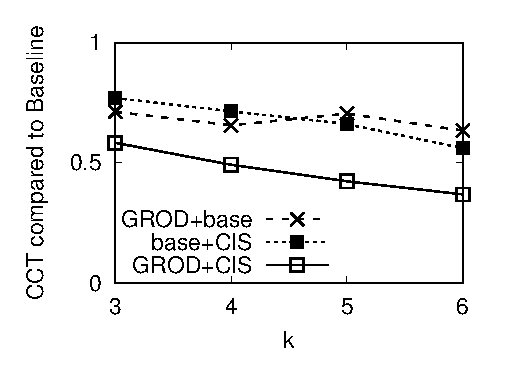
\includegraphics[width=1\textwidth]{28_k_cct.eps}
\caption{CCT compared to Baselinevs. feasible path number $k$ with 2-8 distribution}\label{fig:28_k_cct}
\end{minipage}
\hspace{1mm}
\begin{minipage}[c]{0.23\textwidth}
\centering

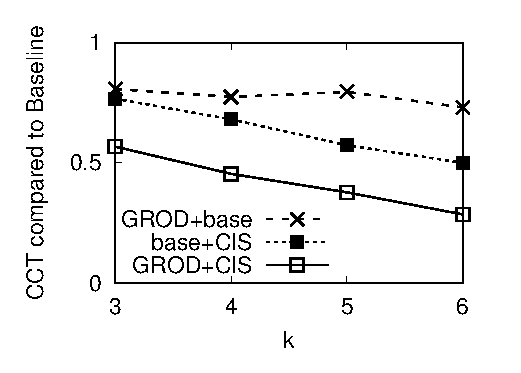
\includegraphics[width=1\textwidth]{normal_k_cct.eps}
\caption{CCT compared to Baseline vs. feasible path number $k$ with normal distribution}\label{fig:normal_k_cct}
\end{minipage}
\hspace{1mm}
\begin{minipage}[c]{0.23\textwidth}
\centering

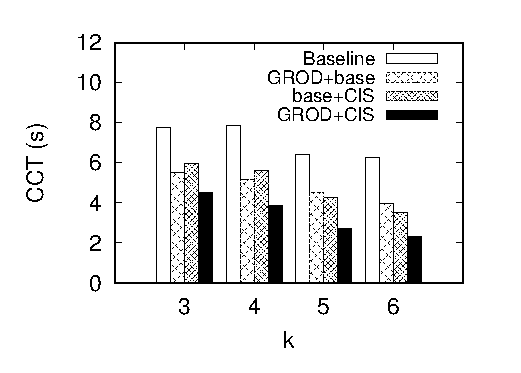
\includegraphics[width=1\textwidth]{28_k_cct_histogram.eps}
\caption{CCT vs. feasible path number $k$ with 2-8 distribution$\qquad\qquad$}\label{fig:28_k_cct_histogram}
\end{minipage}
\hspace{1mm}
\begin{minipage}[c]{0.23\textwidth}
\centering

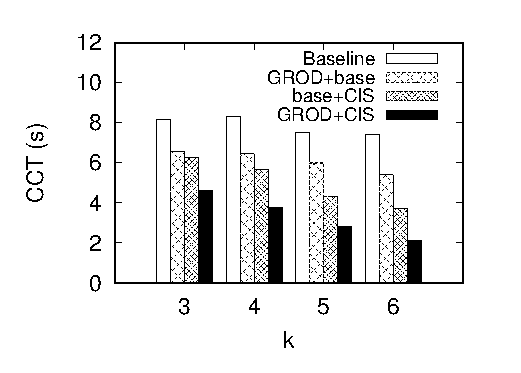
\includegraphics[width=1\textwidth]{normal_k_cct_histogram.eps}
\caption{CCT vs. feasible path number $k$ with normal distribution}\label{fig:normal_k_cct_histogram}
\end{minipage}
\vspace{0cm}
\begin{minipage}[c]{0.23\textwidth}
\centering

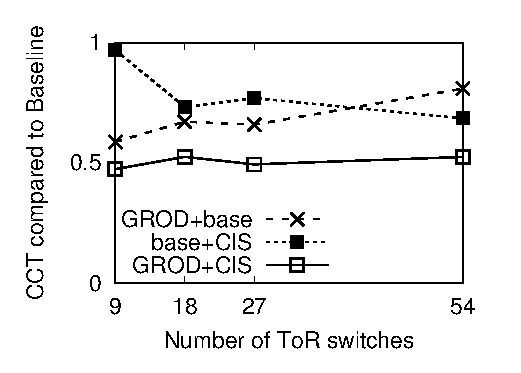
\includegraphics[width=1\textwidth]{28_count_cct.eps}
\caption{CCT compared to Baseline vs. Number of ToR switches with 2-8 distribution}\label{fig:28_count_cct}
\end{minipage}
\hspace{1mm}
\begin{minipage}[c]{0.23\textwidth}
\centering

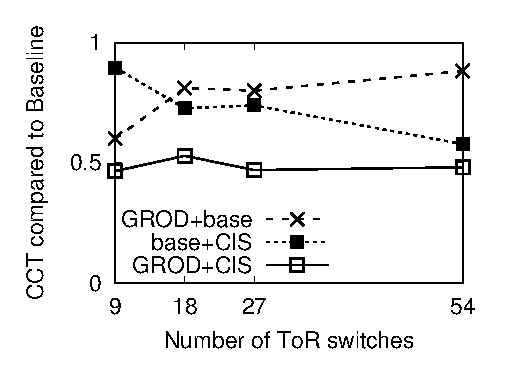
\includegraphics[width=1\textwidth]{normal_count_cct.eps}
\caption{CCT compared to Baseline vs. Number of ToR switches with normal distribution}\label{fig:normal_count_cct}
\end{minipage}
\hspace{1mm}
\begin{minipage}[c]{0.23\textwidth}
\centering

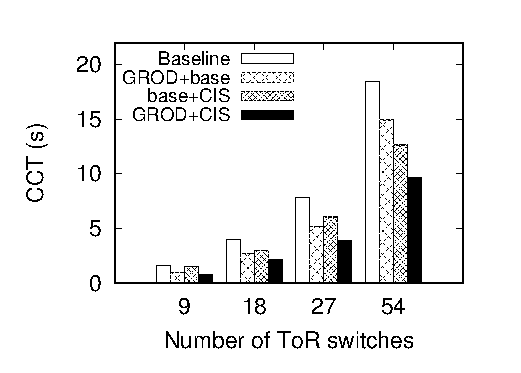
\includegraphics[width=1\textwidth]{28_count_cct_histogram.eps}
\caption{CCT vs. Number of ToR switches with 2-8 distribution$\qquad\qquad$}\label{fig:28_count_cct_histogram}
\end{minipage}
\hspace{1mm}
\begin{minipage}[c]{0.23\textwidth}
\centering
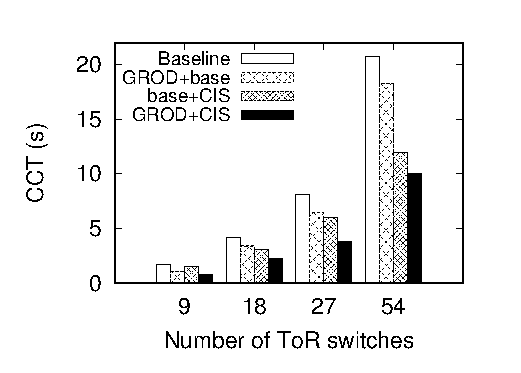
\includegraphics[width=1\textwidth]{normal_count_cct_histogram.eps}
\caption{CCT vs. Number of ToR switches with normal distribution}\label{fig:normal_count_cct_histogram}
\end{minipage}
\vspace{-0.5cm}
\end{figure*}
\begin{figure*}
\centering
\begin{minipage}[c]{0.23\textwidth}
\centering

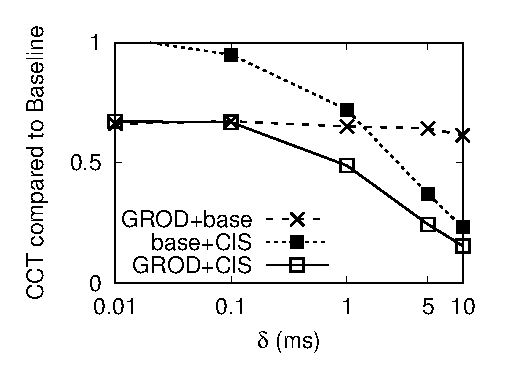
\includegraphics[width=1\textwidth]{28_delta_cct.eps}
\caption{CCT compared to Baseline vs. configuration delay $\delta$ with 2-8 distribution}\label{fig:28_delta_cct}
\end{minipage}
\hspace{1mm}
\begin{minipage}[c]{0.23\textwidth}
\centering

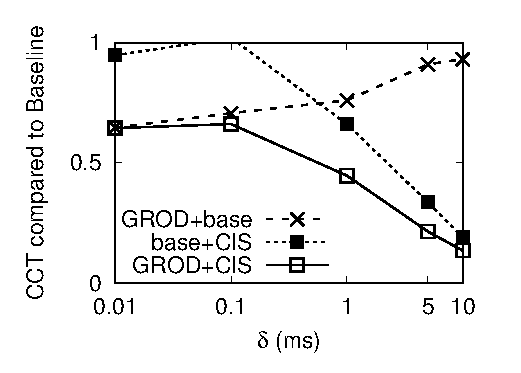
\includegraphics[width=1\textwidth]{normal_delta_cct.eps}
\caption{CCT compared to Baseline vs. configuration delay $\delta$ with normal distribution}\label{fig:normal_delta_cct}
\end{minipage}
\hspace{1mm}
\begin{minipage}[c]{0.23\textwidth}
\centering

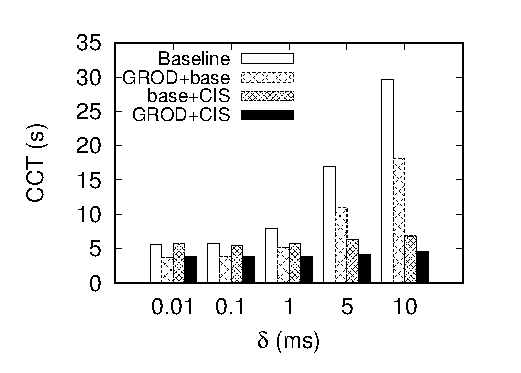
\includegraphics[width=1\textwidth]{28_delta_cct_histogram.eps}
\caption{CCT vs. configuration delay $\delta$ with 2-8 distribution $\qquad\qquad$}\label{fig:28_delta_cct_histogram}
\end{minipage}
\hspace{1mm}
\begin{minipage}[c]{0.23\textwidth}
\centering

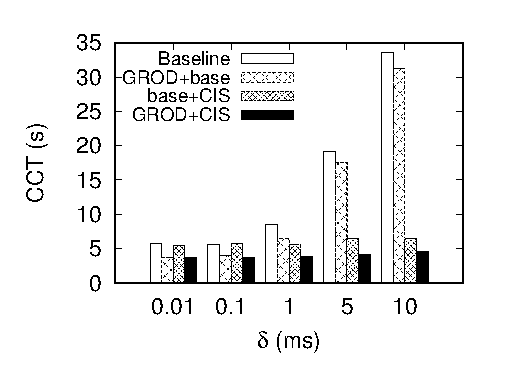
\includegraphics[width=1\textwidth]{normal_delta_cct_histogram.eps}
\caption{CCT vs. configuration delay $\delta$ with normal distribution$\qquad$ $\qquad$}\label{fig:normal_delta_cct_histogram}
\end{minipage}
\vspace{0cm}

\begin{minipage}[c]{0.23\textwidth}
\centering

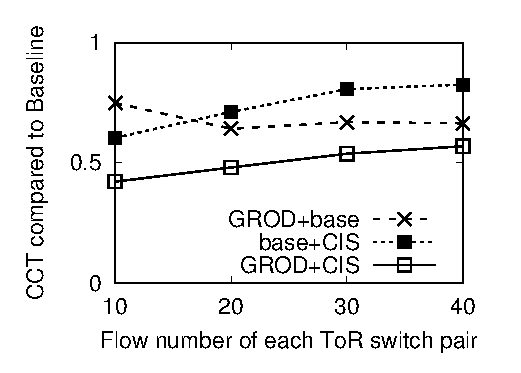
\includegraphics[width=1\textwidth]{28_flow_cct.eps}
\caption{CCT compared to Baseline vs. flow number per ToR pair with 2-8 distribution}\label{fig:28_flow_cct}
\end{minipage}
\hspace{1mm}
\begin{minipage}[c]{0.23\textwidth}
\centering

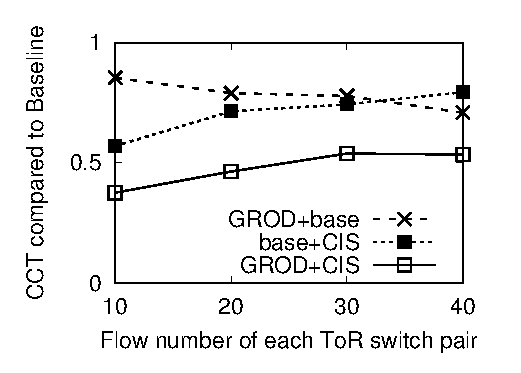
\includegraphics[width=1\textwidth]{normal_flow_cct.eps}
\caption{CCT compared to Baseline vs. flow number per ToR pair with normal distribution}\label{fig:normal_flow_cct}
\end{minipage}
\hspace{1mm}
\begin{minipage}[c]{0.23\textwidth}
\centering

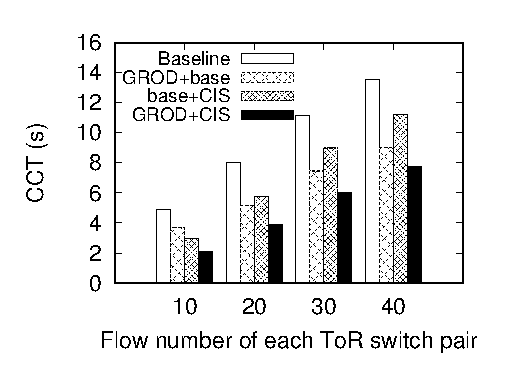
\includegraphics[width=1\textwidth]{28_flow_cct_histogram.eps}
\caption{CCT vs. flow number of each ToR switch pair with 2-8 distribution$\qquad$$\qquad$}\label{fig:28_flow_cct_histogram}
\end{minipage}
\hspace{1mm}
\begin{minipage}[c]{0.23\textwidth}
\centering

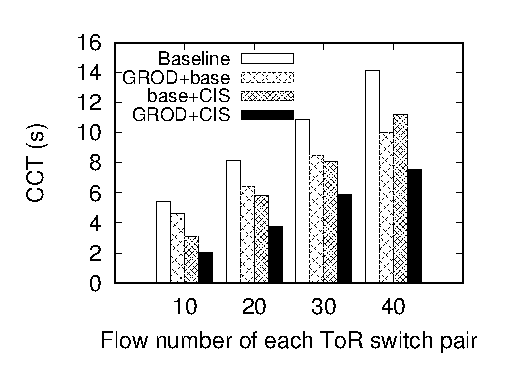
\includegraphics[width=1\textwidth]{normal_flow_cct_histogram.eps}
\caption{CCT vs. flow number of each ToR switch pair with normal distribution$\qquad$$\qquad$}\label{fig:normal_flow_cct_histogram}
\end{minipage}
\vspace{-0.5cm}

\end{figure*}

\subsection{Performance Comparison}
The simulation are performed under four dimensions. Here we illustrate the impacts of four dimensions.

\textbf{Impact of feasible lightpath number $k$:}
To evaluate how the algorithms are influenced by the feasible lightpath number $k$. We fix the other parameters to be defaulted. The result are shown in Figure \ref{fig:28_k_cct}-\ref{fig:normal_k_cct_histogram}, where the horizontal axis is $k$, ranging from 3 to 6. In Fig. \ref{fig:28_k_cct} and \ref{fig:normal_k_cct}, the vertical axis is the coflow completion time (CCT) compared to Baseline. As a result, for all the three algorithms, the CCTs compared to Baseline go down as k increases. For example, in Fig. \ref{fig:normal_k_cct}, the CCT of GROD+CIS compared to Baseline goes down from 0.55 to 0.28. That's because when k goes up, the load on each feasible lightpath is lower and the corresponding duration is smaller. What's more, when $k$ is small, GROD+Base sometimes performs better than Base+CIS. For example, in Fig. \ref{fig:28_k_cct}, when $k=3$, GROD+base will reduce 6\% CCT compared to Base+CIS. However, when $k=6$, GROD+base will increase 6\% CCT compared to base+CIS. That's because our Baseline for CIS is more sensitive to $k$. Our proposed GROD+CIS algorithm can reduce 40-70\% CCT compared to Baseline. Even for base+CIS and GROD+base, our GROD+CIS algorithm can reduce the CCT by 20\%-40\%, especially when $k=6$.

In Fig. \ref{fig:28_k_cct_histogram} and \ref{fig:normal_k_cct_histogram}, the vertical axis is CCT(s). As the feasible lightpath number $k$ increases, there are more lightpaths in the network. As a result, the CCTs of four algorithms decrease. For example, in Fig. \ref{fig:28_k_cct_histogram}, the CCT of baseline goes down from 7.8s to 6.2s when $k$ increases from 3 to 6.

\textbf{Impact of ToR switch number:}
To evaluate how the algorithms are influenced by the ToR switch number. We fix the other parameters to be defaulted. The results are shown in Figure \ref{fig:28_count_cct}-\ref{fig:normal_count_cct_histogram}, where the horizontal axis is the number of ToR switches in the network, ranging from 9 to 54. In Fig. \ref{fig:28_count_cct} and \ref{fig:normal_count_cct}, the vertical axis is the coflow completion time (CCT) compared to Baseline. As a result, the CCT compared to Baseline change little as the number of ToR switches increases for GROD+CIS. But for GROD+base (base+CIS), it goes up (down) as the number of ToR switches increases. What's more, when ToR switch number is small, GROD+base performs better than base+CIS. For example, in Fig. \ref{fig:28_count_cct}, when there are 27 ToR switches, GROD+base will reduce 10\% CCT compared to base+CIS. However, when there are 54 ToR switches, GROD+base will increase 10\% CCT compared to base+CIS. Our proposed GROD+CIS algorithm can reduce 50\% CCT compared to Baseline. Even for base+CIS and GROD+base, our GROD+CIS algorithm can reduce the CCT by 15\%-30\%. That's because our proposed algorithm helps to reduce the CCT by combining coflow scheduling and circuits scheduling.

In Fig. \ref{fig:28_count_cct_histogram} and \ref{fig:normal_count_cct_histogram}, the vertical axis is CCT(s). As the number of ToR switches increases, there are more flows in the network. As a result, the CCTs of four algorithms increase dramatically. For Baseline, the CCT go up from 2s to 18s when ToR switch number increases from 9 to 54.

\textbf{Impact of configuration delay:}
To evaluate how the algorithms are influenced by the configuration delay $\delta$. We fix the other parameters to be defaulted. The result are shown in Figure \ref{fig:28_delta_cct}-\ref{fig:normal_delta_cct_histogram}, where the horizontal axis is $\delta$, ranging from 0.01ms to 10ms. In Fig. \ref{fig:28_delta_cct} and \ref{fig:normal_delta_cct}, the vertical axis is the coflow completion time (CCT) compared to Baseline. As a result, for GROD+CIS and Bseline+CIS, the CCTs compared to Baseline go down as $\delta$ increases. But for GROD+base, it goes up. For example, in Fig. \ref{fig:normal_delta_cct}, the CCT of GROD+CIS compared to Baseline goes down from 0.65 to 0.17. That's because when delta goes up, the reconfiguration times plays an more important role and our proposed CIS algorithm will not change the reconfiguration times, while the baseline of CIS does. For example, in Fig. \ref{fig:normal_delta_cct}, when $\delta=1$, GROD+base and GROD+CIS will reduce approximately 80\% CCT compared to base+CIS and GROD+base.

In Fig. \ref{fig:28_delta_cct_histogram} and \ref{fig:normal_delta_cct_histogram}, the vertical axis is CCT(s). As $\delta$ increases, GROD+base and Baseline dramatically increase the CCT, while base+CIS and GROD+CIS keep stable and much smaller CCT. It shows that our CIS can reduce the reconfiguration times.


\textbf{Impact of flow number per ToR switch pair:}
To evaluate how the algorithms are influenced by the flow number per ToR switch pair. We fix the other parameters to be defaulted. The results are shown in Figure \ref{fig:28_flow_cct}-\ref{fig:normal_flow_cct_histogram}, where the horizontal axis is the flow number per ToR switch pair, ranging from 10 to 40. In Fig. \ref{fig:28_flow_cct} and \ref{fig:normal_flow_cct}, the vertical axis is the coflow completion time (CCT) compared to Baseline. As a result, for base+CIS and GROD+CIS, the CCTs compared to Baseline go up as the flow number per ToR switch pair increases. However, for GROD+base, it goes down, especially for normal distribution. For example, in Fig. \ref{fig:normal_flow_cct}, the CCT of GROD+CIS compared to Baseline goes up from 0.39 to 0.55. But for GROD+base, it goes down from 0.85 to 0.72. That's because when the flow number per ToR switch pair increases, the $\delta$ will be less significant compared to the flow traffic. Just like Fig. \ref{fig:normal_delta_cct_histogram}, when $\delta$ decreases, the CCT compared to Baseline of GROD+CIS and base+CIS increase a bit, but the that of GROD+base keep stable. So it's not because our CIS algorithm doesn't work but essentially because the $\delta$ is less significant compared to the flow traffic when the flow number increases. What's more, when the flow number per ToR switch pair is small, base+CIS sometimes performs better than GROD+base. For example, in Fig. \ref{fig:28_flow_cct}, when the flow number per ToR switch pair is 10, base+CIS reduces 20\% CCT compared to GROD+base. However, when the flow number per ToR switch pair is 40, base+CIS increases 20\% CCT compared to GROD+base. %That's because our base for CIS is more sensitive to the lightpath number. Our proposed GROD+CIS algorithm can reduce 40-60\% CCT compared to Baseline. Even for Baseline+CIS and GROD+base, our GROD+CIS algorithm can reduce the CCT by 20\%-40\%, especially when $flow=6$.

In Fig. \ref{fig:28_flow_cct_histogram} and \ref{fig:normal_flow_cct_histogram}, the vertical axis is CCT(s). As the flow number per ToR switch pair increases, there are more flows in the network. As a result, the CCTs of four algorithms increases. For Baseline in Fig. \ref{fig:normal_flow_cct_histogram}, the CCT goes up from 5.5s to 14s when  the flow number per ToR switch pair increases from 10 to 40.

\subsection{Running Time}
In this part, we evaluate how the feasible lightpath number $k$ and ToR switch number can influence the running time. The results are shown in Fig. \ref{fig:28_k_time_histogram} and \ref{fig:28_count_time_histogram}, where the vertical axis is running time. In Fig. \ref{fig:28_k_time_histogram}, as $k$ increases, the running time increases too. But compared to the Fig. \ref{fig:28_count_time_histogram}, the running time increases dramatically when the number of ToR switches increases. That's because the lightpath number is $O(n^2)$ for the number of ToR switches while $k$ can only change the number of lightpaths linearly.

\begin{figure}
\centering
\begin{comment}
\begin{minipage}[c]{0.23\textwidth}
\centering
\includegraphics[width=1\textwidth]{28_k_time.eps}
\caption{Running time compared to Baseline vs. feasible lightpath number $k$ with 2-8 distribution}\label{fig:28_k_time}
\end{minipage}
\hspace{1mm}
\end{comment}
\begin{minipage}[c]{0.23\textwidth}
\centering

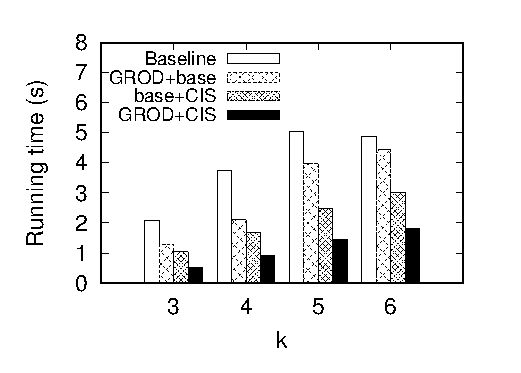
\includegraphics[width=1\textwidth]{28_k_time_histogram.eps}
\caption{Running time vs. feasible lightpath number $k$ with 2-8 distribution}\label{fig:28_k_time_histogram}
\end{minipage}
\vspace{-0.3cm}
\begin{comment}
\begin{minipage}[c]{0.23\textwidth}
\centering

\includegraphics[width=1\textwidth]{28_count_time.eps}
\caption{Running time compared to Baseline vs. ToR switch number with 2-8 distribution}\label{fig:28_count_time}
\end{minipage}
\end{comment}
\hspace{1mm}
\begin{minipage}[c]{0.23\textwidth}
\centering

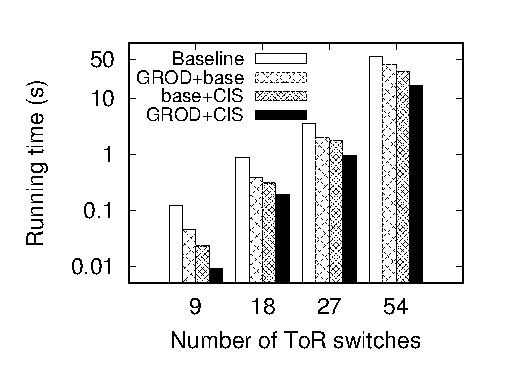
\includegraphics[width=1\textwidth]{28_count_time_histogram.eps}
\caption{Running time vs. ToR switch number with 2-8 distribution}\label{fig:28_count_time_histogram}
\end{minipage}
\vspace{-0.3cm}


\end{figure}

%\subsection{Conclusion}
%Our GROD+CIS algorithm can reduce the CCT by 40-80\% compared to Baseline in four dimensions. The two hybrid algorithms, GROD+base and base+CIS, achieve the CCTs in the middle of Baseline and GROD+CIS, which shows the effectiveness of both of steps. Because of the space is limited, we do not repeat in detail.
